\documentclass{report}
\usepackage[margin=1in]{geometry}
\usepackage{cite}
\usepackage{amsmath,amssymb,amsfonts}
\usepackage{algorithmic}
\usepackage{graphicx}
\usepackage{textcomp}
\usepackage{tabstackengine}
\usepackage{xcolor}
\usepackage{subcaption}
\usepackage{cuted}

\begin{document}
	\tableofcontents
	\section*{Preface}
	The work contained in this PDF is an attempt on my part to synthesize the entirety of my understanding of monolithic, or "fully integrated" power conversion. I am doing this to improve my technical writing and communication abilities, in addition to furthering my own understanding of the material on which I write, hopefully someone can make some use of these writings. At the time of writing this, I have no idea how long this will take, or if I will ever actually complete this work, but I hope to make some progress.
	
	The current plan for writing this is to write it in such a way that it appeals to the reader from first principles, as much of the work and theory presented is without real world validation, or chip fabrication. The required background on the part of the reader is essentially that they understand:
	\begin{itemize}
		\item Circuit theory - Resistors, capacitors, inductors, nodal analysis, etc.
		\item Electronics - Comfortable with diodes, and transistors, along with there various uses. Transistors in saturation, triode, on resistance of transistors, gate capacitance, etc.
		\item Mathematics - Differential equations, laplace transforms, frequency domain analysis.
	\end{itemize}
	Provided the reader has background in these topics, it is my hope that my communication abilities are sufficient enough to make the following writings understandable.
	   
	\chapter{Introduction}
	
	
	\chapter{Switched Capacitor Power Converters - Fundamentals}
Switched Capacitor Power Converters (SCPCs)
	\section{Four Terminal Model}
	The four terminal model is the simplest place to begin the explanation of how SCPCs operate. In this, the circuit in Fig. \ref{fig:sccell1} represents the most fundamental unit of the SCPC, with 4 different voltages being connected to a single capacitor through switches. This capacitor is referred to frequently as the flying capacitor in much of the literature, presumably because both the top and bottom plate voltages vary over time, and the capacitor is not "grounded". 
	
\begin{figure}
	\centering
	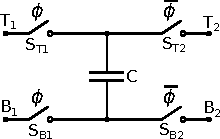
\includegraphics[width=0.4\linewidth]{4Terminal/Figures/SCCell_1.pdf}
	\caption{The fundamental Switched Capacitor cell.}
	\label{fig:sccell1}
\end{figure}
	
	The four terminal device operates in two different phases, referred to as phases 1 and 2. Phase one can be seen in Fig. \ref{fig:Phase1}, where the clock ($\phi$) is high, causing switches $S_{T1}$ and $S_{B1}$ to be enabled. This results in a short circuit between the top plate and $V_{T1}$ (the top terminal voltage in phase 1), and a short between $V_{B1}$ and the bottom plate of the flying capacitor. The circuit corresponding to phase 2 can be seen in Fig. \ref{fig:Phase2}, where the top plate is shorted to $V_{T2}$ and the bottom plate to $V_{B2}$.
	
	This circuit effectively delivers current from ${T2}$ to ${T1}$ as well as moving current from ${B2}$ to ${B1}$. This occurs through the mechanism of stored charge on the flying capacitor. Consider phase 1, where the voltage drop across the capacitor ($V_{C}$) is $V_{T1} - V_{B1}$. In phase 2 however, the voltage drop across the capacitor is $V_{T2} - V_{B2}$, resulted in a change in voltage, and thus a charge flow ($Q$) equal to $Q = C_{Fly}(V_{T2} - V_{B2} - V_{T1} + V_{B1})$.
	
	\begin{figure}
		\begin{subfigure}{0.4\linewidth}
			\centering
			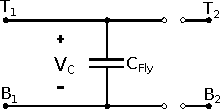
\includegraphics[width=\linewidth]{4Terminal/Figures/Phase1.pdf}
			\caption{Phase 1.}
			\label{fig:Phase1}
		\end{subfigure}
		\hfill
		\begin{subfigure}{0.4\linewidth}
			\centering
			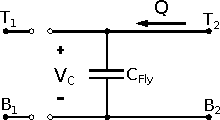
\includegraphics[width=\linewidth]{4Terminal/Figures/Phase2.pdf}
			\caption{Phase 2.}
			\label{fig:Phase2}
		\end{subfigure}
		\caption{Different phase representations of the circuit in Fig. \ref{fig:sccell1}}
	\end{figure}
	
	This charge flow will then occur in opposite value in the first phase. These charge transfers occur repeatedly, determined by the switching frequency ($f_{SW}$) of the clock. Given the switching frequency, the steady state/average current delivered by the flying capacitor can be calculated as,
	\begin{equation}
		I_{CFly} = Qf_{SW} = C_{Fly}f_{Sw}(V_{T2} - V_{B2} - V_{T1} + V_{B1}),
	\end{equation} 
	which in this case is the power moved between the different voltage domains. Consider the structure in the case where it is operating as a buck converter, corresponding to Fig. \ref{fig:Buck}. The output current will be comprised of the current flowing through $S_{T1}$ and $S_{B2}$, which in this case is,
	\begin{equation}
		I_{OUT} = 2I_{CFly} = 2C_{Fly}f_{Sw}(V_{IN} - 2V_{OUT}),
	\end{equation} 
	while the input current is,
	\begin{equation}
		I_{IN} = I_{CFly} = C_{Fly}f_{Sw}(V_{IN} - 2V_{OUT}).
	\end{equation}
	\begin{figure}
		\centering
		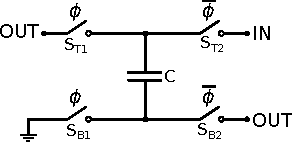
\includegraphics[width=0.5\linewidth]{4Terminal/Figures/Buck.pdf}
		\caption{Switched capacitor cell in the buck configuration.}
		\label{fig:Buck}
	\end{figure}
	From these two equations, the power conversion efficiency ($\eta$) can be calculated by assessing the ratio between the output and input power,
	\begin{equation}
		\eta = \frac{P_{OUT}}{P_{IN}},
	\end{equation}	
	given that $P_{OUT} = V_{OUT}I_{OUT}$, and $P_{IN} = V_{IN}I_{IN}$, this resolves to,
	\begin{equation}
		\eta = \frac{2V_{OUT}}{V_{IN}}.
	\end{equation} 
	This indicates a clear relationship between the input and output voltages, where the conversion ratio ($\gamma$) determines the efficiency of the structure. Unfortunately, this is presents a very large challenge for SCPCs, as many applications require different conversion ratios to operate optimally, resulting in an inevitable loss in efficiency.
	
	An equivalent steady state model can also be developed, using resistors and dependent voltage sources, seen in Fig. \ref{fig:ResModelBasic} where $R_{Fly} = \frac{1}{C_{Fly}f_{Sw}}$.
	\begin{figure}
		\centering
		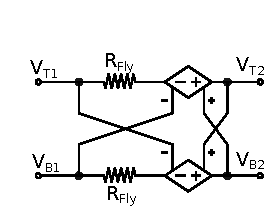
\includegraphics[width=0.4\linewidth]{4Terminal/Figures/CellRes_SSL_Basic.pdf}
		\caption{Resistive steady state model of the circuit in, Fig. \ref{fig:sccell1}.}
		\label{fig:ResModelBasic}
	\end{figure}
	
	\subsection{Parasitic Capacitance}
	It must be noted that the prior model of the flying capacitor presented was a simplification of the real model. Actual flying capacitors designed on-chip have stray or parasitic capacitances, where the top and bottom plate are capacitively coupled to other structures within the IC. Most notably is usually the capacitance between the bottom plate of $C_{Fly}$ and the substrate.
	
	These stray capacitances are almost always directly proportional to the flying capacitor by some fixed ratio. This can be factored into the model of the flying capacitor, where the bottom plate parasitic ratio is $\alpha_B$ and the top plate is $\alpha_T$, as in Fig. \ref{fig:sccell}. The details surrounding these parasitic capacitances will be covered in Chap. \ref{CH:FlyingCap}.
	
	\begin{figure}
		\centering
		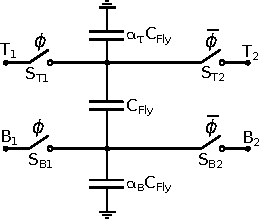
\includegraphics{4Terminal/Figures/SCCell.pdf}
		\caption{Switched capacitor cell incorporating effects of $\alpha_B$ and $\alpha_T$.}
		\label{fig:sccell}
	\end{figure}
	
	The impact of $\alpha_B$ and $\alpha_T$ on the four terminal model will now be covered. Consider first the impact of $\alpha_T$, in the first phase it is charged to $V_{T1}$, while in the second it is charged to $V_{T2}$. This corresponds to a charge flow of $Q_{\alpha T} = C_{Fly}\alpha_T(V_{T2} - V_{T1})$, which as a steady state current is, $I_{\alpha T} = f_{SW}C_{Fly}\alpha_T(V_{T2} - V_{T1})$. Similarly the current flow associated $\alpha_B$ is $I_{\alpha B} = C_{Fly}\alpha_B(V_{B2} - V_{B1})$.
	
	From this, the current from ${T2} \rightarrow {T1}$ is, 
	\begin{equation}
		I_{T2,T1} = I_{CFly} + I_{\alpha_T} = f_{SW}C_{Fly}\left((V_{T2} - V_{B2} - V_{T1} + V_{B1}) + \alpha_T(V_{T2} - V_{T1})\right),
	\end{equation}
	while the current from ${B2} \rightarrow {B1}$ is,
	\begin{equation}
		I_{B2,B1} = -I_{CFly} + I_{\alpha_B} = f_{SW}C_{Fly}\left((V_{B2} - V_{T2} - V_{B1} + V_{T1}) + \alpha_B(V_{B2} - V_{B1})\right).
	\end{equation}
	The resistive equivalent circuit can be seen in Fig. \ref{fig:resModel}, which adds the effects of the parasitic capacitance to Fig. \ref{fig:ResModelBasic}.
	\begin{figure}
		\centering
		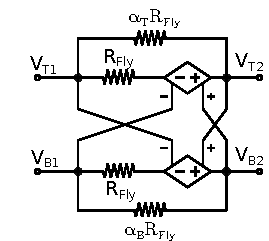
\includegraphics[width=0.4\linewidth]{4Terminal/Figures/CellRes.pdf}
		\caption{Resistive steady state model of the circuit in Fig. \ref{fig:sccell}. Note that $R_{Fly} = \frac{1}{C_{Fly}f_{Sw}}$.}
		\label{fig:resModel}
	\end{figure}
	
	\subsection{Switch Resistance}
	The prior models assumed that the switches had no effective resistance. This only models the behaviour correctly when the frequency is low enough that the capacitors can fully charge and discharge. In reality, the switches have some finite resistance $R_{SW}$, which will degrade the performance of the converter.
	
	To begin, consider Fig. \ref{fig:Phase1Res}, in which the switch resistance is included in the phase 1 circuit. Here we can see that the top and bottom plate voltages ($V_{TP1}$ and $V_{BP1}$) are separated from $T_1$ and $B_1$ by an equivalent switch resistance element. In order to describe $V_{TP1}$ and $V_{BP1}$ with respect to time, nodal analysis must be used. 
	
	\begin{figure}
		\centering
		\begin{subfigure}{0.35\linewidth}
			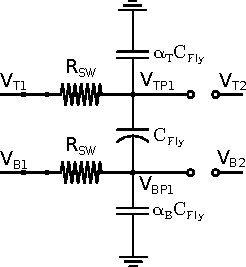
\includegraphics[width=\linewidth]{4Terminal/Figures/Phase1EQ.pdf}
			\caption{Phase 1.}
			\label{fig:Phase1Res}
		\end{subfigure}
		\hfill
		\begin{subfigure}{0.35\linewidth}
			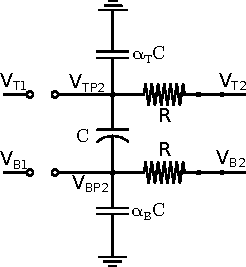
\includegraphics[width=\linewidth]{4Terminal/Figures/Phase2EQ.pdf}
			\caption{Phase 2.}
			\label{fig:Phase2Res}
		\end{subfigure}
	\caption{Circuit level equivalents of the circuit in Fig. \ref{fig:Phase1} and \ref{fig:Phase2}.}
	\end{figure}
	
	The first nodal analysis occurs at node $V_{TP1}$, yielding,
	\begin{equation}
		s\alpha_T C_{Fly} V_{TP1} + sC_{Fly}(V_{TP1} - V_{BP1}) + \frac{V_{TP1} - V_{T1}}{R_{SW}} = 0.
	\end{equation}
	Similarly, a nodal analysis at the bottom plate node yields,
	\begin{equation}
		s\alpha_B C_{Fly} V_{BP1} + sC_{Fly}(V_{BP1} - V_{TP1}) + \frac{V_{BP1} - V_{B1}}{R_{SW}} = 0.
	\end{equation}
	The goal of the nodal analysis is to identify the dominant poles of the circuit so that a first order approximation can be used to describe the voltage. For simplicity we set $V_{B1} = 0$, though the choice of $V_{T1}$ or $V_{B1}$ is arbitrary. The resulting transfer function for $V_{TP1}$ is, 
	\begin{equation}
		V_{TP1} = \frac{sV_CCR(\alpha_BCRs + 1)}{s^2C^2R^2(\alpha_B + \alpha_T + \alpha_B\alpha_T) + sCR(2+\alpha_B+\alpha_T) + 1},
	\end{equation}
	the dominant pole of the circuit is located at, $s \approxeq \frac{2}{RC(4 + \alpha_B + \alpha_T)}$. Using the dominant pole, a first order approximation of the exponential decay can be used. For example, the exponential first order decay at node $V_{TP1}$ is,
	\begin{equation}
		V_{TP1}(t) = V_{initial}\exp\left(\frac{-t}{\tau}\right) + V_{T1}\left(1 - \exp\left(\frac{-t}{\tau}\right)\right),
	\end{equation}
	where $\tau$ is determined by the dominant pole,
	\begin{equation}
		\tau \approxeq \frac{2}{RC(4 + \alpha_B + \alpha_T)}.
	\end{equation}
	Given that each phase occurs for time equal to half of the switching period, the final voltage at the end of the time step is,
	\begin{equation}
		V_{TP1,final} = V_{TP1}\left(t=\tfrac{T_{SW}}{2}\right) = V_{initial}\exp\left(\frac{-T_{SW}}{2\tau}\right) + V_{T1}\left(1 - \exp\left(\frac{-T_{SW}}{2\tau}\right)\right).
	\end{equation}
	A substitution can be made for the exponential decay, where
	\begin{equation}
		A = \exp\left(\frac{-T_{SW}}{2\tau}\right) = \exp\left(\frac{-1}{f_{SW}RC(4+\alpha_B+\alpha_T)}\right).
	\end{equation}
	The corresponding equations for the final voltages and their relationship is then as follows for all 4 nodes,
	\begin{equation}
		V_{TP1}^f = AV_{TP1}^i + (1-A)V_{T1},
	\end{equation}
	\begin{equation}
		V_{BP1}^f = AV_{BP1}^i + (1-A)V_{B1},
	\end{equation}
	\begin{equation}
		V_{TP2}^f = AV_{TP2}^i + (1-A)V_{T2},
	\end{equation}
	\begin{equation}
		V_{BP2}^f = AV_{BP2}^i + (1-A)V_{B2}.
	\end{equation}
	
	Next, to determine the initial conditions, consider the value of $V_{C}$. During the start of phase 1, $V_C$ will be directly related to the voltage drop across the capacitor at the end of phase 2 $V_C = V_{TP2}^f - V_{BP2}^f$. The initial conditions can then be acquired using Fig. \ref{fig:Phase1_t0}, which represents Fig. \ref{fig:Phase1Res} immediately at the start of Phase 1. From this,
	\begin{equation}
		V_{TP1}^i = \frac{V_{T1} + V_{B1} + V_{TP2}^f - V_{BP2}^f}{2},
	\end{equation}
	while 
	\begin{equation}
		V_{BP1}^i = \frac{V_{T1} + V_{B1} + V_{TP2}^f - V_{BP2}^f}{2}.
	\end{equation}
	\begin{figure}
		\centering
		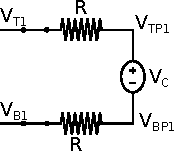
\includegraphics[width=0.3\linewidth]{4Terminal/Figures/Phase1EQ_t=0.pdf}
		\caption{Electrical equivalent to Fig. \ref{fig:Phase1Res} at t=0.}
		\label{fig:Phase1_t0}
	\end{figure}
	A similar procedure can be followed to acquire the initial conditions for phase 2, where
	\begin{equation}
		V_{TP2}^i = \tfrac{V_{TP1}^f - V_{BP1}^f + V_{T2} + V_{B2}}{2},
	\end{equation}
	and
	\begin{equation}
		V_{BP2}^i = \tfrac{V_{BP1}^f - V_{TP1}^f + V_{T2} + V_{B2}}{2}.
	\end{equation}
	These equations can be substituted into the equations for the final voltages, to yield the solved equations,
	\begin{equation}
		V_{TP1}^f = V_{T1} + \Delta V, 
	\end{equation}
	\begin{equation}
		V_{BP1}^f = V_{B1} - \Delta V,
	\end{equation}
	\begin{equation}
		V_{TP2}^f = V_{T2} - \Delta V,
	\end{equation}
	and
	\begin{equation}
		V_{BP2}^f = V_{B2} + \Delta V
	\end{equation}
	where 
	\begin{equation}
		\Delta V = \frac{A(V_{B1} - V_{T1} - V_{B2} + V_{T2})}{2(A+1)}.
	\end{equation}
	From this, the 4 terminal device model in \ref{fig:cellresfsl} can be generated, which can easily be implemented in pspice, verilogA, or a number of other simulators. The accuracy of the model was tested using pspice, where the circuit in Fig. \ref{fig:sccell} was implemented using switches with on resistance. The resulting comparisons run can be seen in Fig. \ref{} - \ref{}, in which the models appear quite accurate for a broad range of conditions. 
	
\begin{figure}
	\centering
	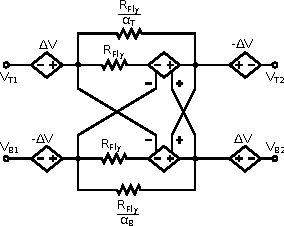
\includegraphics[width=0.5\linewidth]{4Terminal/Figures/CellRes_FSL.pdf}
	\caption{Steady state 4 terminal model incorporating switch resistance.}
	\label{fig:cellresfsl}
\end{figure}
	
	It should be noted however, that while the model in Fig. \ref{fig:cellresfsl} is compact, it does not lend itself nicely to hand calculation. Instead, the circuit in Fig. \ref{fig:cellresfsl2} is more appropriate, where 
	\begin{equation}
		R_{1} = \frac{A+1}{fCR(1-A(1-\alpha_T))},
	\end{equation}
	and
	\begin{equation}
		R_{2}  = \frac{A+1}{fCR(1-A(1-\alpha_B))}.
	\end{equation}
	\begin{figure}
		\centering
		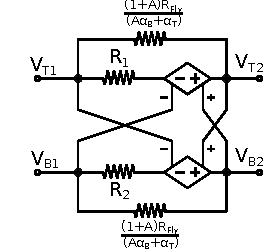
\includegraphics[width=0.4\linewidth]{4Terminal/Figures/CellRes_FSL_2.pdf}
		\caption{Equivalent circuit to \ref{fig:cellresfsl}.}
		\label{fig:cellresfsl2}
	\end{figure}
	
	
	\subsection{Frequency Domain Model}
	Depending on the way in which the SCPCs are used, there is a need to develop models which approximate the impedance of the structure. If it is assumed that the switching frequency of the structure is constant with respect to time, then the model in Fig. \ref{} provides an excellent first order approximation. The added impedance between the top and bottom plate is a result of the instantaneous connections which occur in both Phase 1 and Phase 2. As the converter is split between these two phases 50\% of the time, the impedance of the elements is doubled. 
	
	
	\section{SCPC Topologies}
	There are numerous topologies which are used in SCPC design in order to implement different voltage conversion ratios. While the SC cell in \ref{} is capable of implementing 2:1 or 1:2 conversion, many applications require different voltage conversion ratios, facilitating different architectures.
	\subsection{Dickson}
	The Dickson topology can be understood from the diagram in \ref{fig:NDickson}, in which a generic $N$ stage Dickson is shown. The resulting voltage conversion ratio is N+1:1 in a buck conversion ratio, and 1:N+1 in a boost.
	
	\begin{figure}
		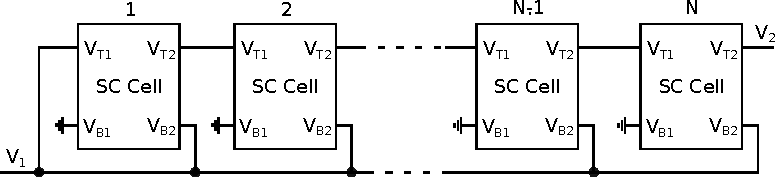
\includegraphics[width=\linewidth]{4Terminal/Figures/NDickson.pdf}
		\caption{N-stage Dickson converter comprised of the cells in \ref{}.}
		\label{fig:NDickson}
	\end{figure}
	
	The benefits of the structure are that it has a constant voltage stress across all of its transistors, with increasing stress across its capacitors per stage. The output resistance and efficiency can be acquired using the models in \ref{} and \ref{}, though the choice to include switch resistance depends on the operation of the converter.
	\subsection{Series Parallel}
	A diagram of the Series Parallel topology is in Fig. \ref{} for a generic $N$ stages. Similar to the Dickson, the resulting conversion ratio is N+1:1 in a buck configuration, and 1:N+1 in a boost.
	
	The structure features a constant stress across the flying capacitors, with switch voltage stresses depending on $N$.
	\subsection{XXXX}
	In the context of monolithic SCPCs, the XXXX configuration can be seen in Fig. \ref{}, with its equivalent circuit in Fig. \ref{}.
	
	The structure features a constant stress across the flying capacitors, in addition to constant stress across the transistors.
	
	\subsection{Fractional Converters}
	\subsection{Fibonacci and Exponential}
	The Fibonacci, charge pump refers to the architecture in \ref{}, in which the VCR follows the Fibonacci sequence. The exponential charge pump architecture refers to Fig. \ref{}, in which the VCR $= 2^N$. 
	
	Both these architectures feature voltage, and capacitor stresses which are dependent on the number of stages. 

	\subsection{Hybrid Architectures}
	Here are various SCPC architectures which are potentially useful in a number of scenarios, depending entirely on the technology, and the desired conversion ratio.
	
		
	
	\chapter{Flying Capacitor Design}
	\label{CH:FlyingCap}
	\chapter{Transistor Considerations}
	\chapter{Time Interleaving}
	\chapter{Charge Reuse}
	\chapter{Stage Outphasing}
	\chapter{Reconfigurable Architectures}
	\chapter{Advanced Models}
There are a number of other important effects not accounted for by the models in Chap. \ref{chap:Fundamentals}. The chapter developed functioning steady state models, but no time, or frequency domain models were developed. In addition, there are a number of technology dependent effects which can impact performance which need to be considered.
\section{Transistor Leakage}
One increasingly important design variable at smaller technology nodes is the impact of leakage between the various nodes of the transistors.
\subsection{Sub-Threshold Leakage}
Sub-Threshold leakage refers to the current that flows between the drain and the source of the transistor when the transistor is turned off. 

The analysis begins by assuming that the flying capacitor cell almost completely charges and discharges each cycle. The assumption is based on the fact that this is the region in which the leakage effects have the largest impact on performance.

Next, the impact on the SCPC can be understood by considering the various phases of the converter, as in Fig. \ref{}. In phase 1, $V_{TP1} = V_{T1}$, resulting in a $V_{DS}$ of $V_{T2} - V_{T1}$ across $S_{T2}$. Similarly, $V_{BP1} = V_{B1}$, making $V_{DS} = V_{B2} - V_{B1}$ for $S_{B2}$. Likewise in phase 2, the $V_{DS}$ of $S_{T1} = V_{T2} - V_{T1}$, while the $V_{DS}$ of $S_{B1} = V_{B2} - V_{B1}$. 

Assuming the phases occupy equal portions of the period, then 
\begin{equation}
	I_{Leak,T2,T1} = \frac{I_{Leak,ST2} = I_{Leak,ST1}}{2},
\end{equation}
where $I_{VDS,ST2}$ denotes the drain to source leakage of $S_{T2}$, while 
\begin{equation}
	I_{Leak,B2,B1} = \frac{I_{Leak,SB2} = I_{Leak,SB1}}{2},
\end{equation}
which get incorporated into the model as in Fig. \ref{}. In order to acquire their leakage values, the transistors comprising switches must be simulated at their corresponding $V_{DS}$. Additionally, if the leakage varies substantially with $V_{DS}$, then it is advisable to include a voltage dependence. Lastly, there is temperature variation in the sub-threshold leakage which will impact performance and may need to be considered.

\subsection{Gate Oxide}

\section{Frequency Domain Model}
In order to incorporate SCPC into many designs and applications, their frequency domain model is required. To begin, consider the instantaneous connections between the various terminals of the converter. 

The circuits in Fig. \ref{}, provides an illustration of the instantaneous connections between nodes $V_{T2}$ and $V_{B2}$ as well as $V_{T1}$ and $V_{B1}$. This can immediately be incorporated into the model in Fig. \ref{}, resulting in Fig. \ref{}. 

Next, the frequency domain model for the current flow between $V_{T2}$ and $V_{T1}$ can be generated. 

Depending on the way in which the SCPCs are used, there is a need to develop models which approximate the impedance of the structure. If it is assumed that the switching frequency of the structure is constant with respect to time, then the model in Fig. \ref{} provides an excellent first order approximation. The added impedance between the top and bottom plate is a result of the instantaneous connections which occur in both Phase 1 and Phase 2. As the converter is split between these two phases 50\% of the time, the impedance of the elements is doubled. 
	
	
	\chapter{Control}
	\chapter{Design Examples}
	\chapter{Continuously Scalable}
	
\end{document}